\documentclass[a4paper, 12pt]{article}
\usepackage[utf8]{inputenc}
\usepackage[T1]{fontenc}
\usepackage{textcomp, color, amsmath, amssymb, tikz, subfig, float, mathrsfs}
\usepackage{xcolor}
\usepackage{amsfonts}
\usepackage{graphicx}
\usepackage{listings}
\usepackage{ragged2e}
\usepackage{amsmath}
\usepackage[export]{adjustbox}
\usepackage[]{esint}
\usepackage{hyperref}
\usepackage[skins,theorems]{tcolorbox}
\usepackage{cite}
\usepackage{algorithm}
\usepackage{algorithmicx}
\usepackage{algpseudocode}
\usepackage{subfig}% http://ctan.org/pkg/subfig
\usepackage{hyperref}
\usepackage{setspace}
\newsubfloat{figure}
%Tikzcommands
\usepackage{tikz}
\usetikzlibrary{shapes.geometric, arrows}
\tikzstyle{startstop} = [rectangle, rounded corners, minimum width=3cm, minimum height=1cm,text centered, draw=black, fill=red!30]
\tikzstyle{io} = [trapezium, trapezium left angle=70, trapezium right angle=110, minimum width=3cm, minimum height=1cm, text centered, draw=black, fill=blue!30]
\tikzstyle{process} = [rectangle, minimum width=3cm, minimum height=1cm, text centered, draw=black, fill=orange!30]
\tikzstyle{decision} = [diamond, minimum width=3cm, minimum height=1cm, text centered, draw=black, fill=green!30]
\tikzstyle{arrow} = [thick,->,>=stealth]




\tcbset{highlight math style={enhanced,
  colframe=red,colback=white,arc=10pt,boxrule=0.5pt, hbox}}

\definecolor{lightgray}{gray}{0.75}

\newcommand\greybox[1]{%
  \vskip\baselineskip%
  \par\noindent\colorbox{lightgray}{%
    \begin{minipage}{\textwidth}#1\end{minipage}%
  }%
  \vskip\baselineskip%
}
	
\newcommand{\vertfig}[2][]{%
  \begin{minipage}{5in}\subfloat[#1]{#2}\end{minipage}}
  
\newcommand{\horizfig}[2][]{%
  \begin{minipage}{3in}\subfloat[#1]{#2}\end{minipage}}

\linespread{1.5}
\begin{document}



\author{Kristian Tuv}
\title{FYS3710  EPR}
\maketitle

\section{Innledning}
I denne oppgaven skal vi bruke Elektron Paramagnetisk Resonans spektroskopi til \\
a) Deteksjon av H og D-atomer i bestrålt vann og tungtvann\\
b) Dosebestemmelse av bestrålte nitroglyserintabletter fra kjellerulykken i 1982

\section{Teori}
Et elektron har et magnetisk moment
$$\mu = -g\beta S$$
der g er en karakterisisk konstant og $\beta $ er Bohrmagnetonet $e\hbar /2me$ og S er spinnet.\\
Elektronet vil påvirkes av et ytre magnet felt og rette seg etter magnetfeltet med spinnet enten parallellt eller antiparallellt.\\
Disse to tilsstanden har ikke samme energi og energidifferansen er
$$\Delta E = g\beta B$$
Der B er den magnetiske flukstettheten. Det vil alltid være noen flere elektroner i tilstanden forbundet med lavest energi.
Vi kan indusere overganger mellom de to energitilstandene ved å utsette spinnsystemet for elektronmagnetisk stråling med energi $$h \nu  = \Delta E = g\beta B$$
der $\nu$ er frekvensen til strålingen. Dette kalles resonansbetingelsen.\\
Sannsynligheten for for å få overganger mellom tilstandene er den samme uansett hvilken vei overgangen skjer, men fordi det er flere elektroner i den laveste energi tilstanden vil vi få en netto energiabsorbsjon. Det er denne energiabsorbsjonen som utgjør et  EPR-signal.\\
Intensiteten av energiabsorpsjonener proposjonalt med antallet uparede elektroner i prøven som studeres Arealet er ofte proporsjonalt med absorpsjonskurvens ampitude, slik at det under slike forhold rekker å måle absorpsjonskurvens amplituder i steden for å integrere spektret for å finne arealet.\\
EPR spekteret er også avhengig av om det finnes kjerner i nærheten av elektronet som kan påvirke det magnetiske momentet til elektronet. Slike vekselvirkninger fører til at den enkle energiabsorbsjonslinjen en får ved resonans fra elektronet alene blir splittet opp på en måte som er karakteristisk for hvilke kjerner elektronet vekselvirker med, antallet av slike kjerner, samt styrken av koplingen til de forskjellige kjernene.

\section{Gjennomføring del a}
Svovelsyre fra en blanding av tungtvann og normalt vann dryppes med en dråpeteller ned i et bad med flytende nitrogen (T=77 K). Iskulene som dannes bestråles med røntgenstråling (60 kV / 40 mA) i ca. 10 minutter og EPR spektrene tas deretter opp ved 77 K. Vi leser av magnetfelt verdiene på toppene i spekeret, og bruker disse verdiene til ål beregne
\section{Oppgaver del a}
\subsection*{1}%1
\begin{figure}[H]
\centering
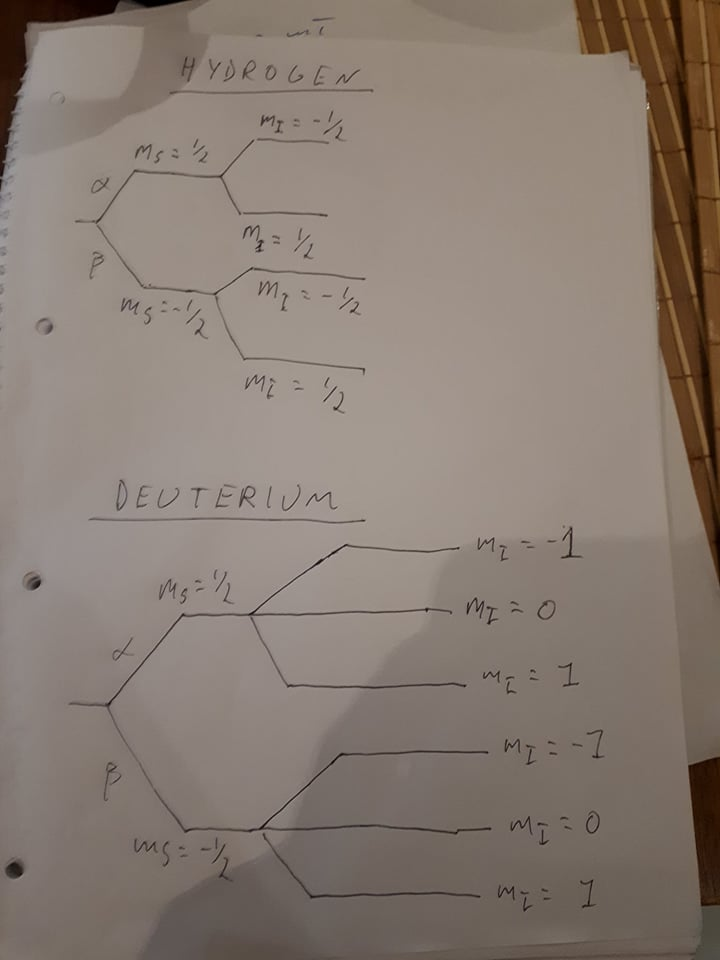
\includegraphics[scale=.5]{/Users/Tuv/Documents/UiO/H17/FYS3710/EPR/oppgave1.jpg}
\caption{Energidiagram}
\end{figure}
\subsection*{2}%2
$a = (2\mu_{0} /3)g_N\beta_{N}|\Psi (0)|^2$\\
Det eneste som er ulikt for $a_H$ og $a_D$ er $g_N$, så 
$$\frac{a_H}{a_D}=5.585/0.857 = 6.517$$
\subsection*{3 og 4}%4
\begin{figure}[H]
\centering
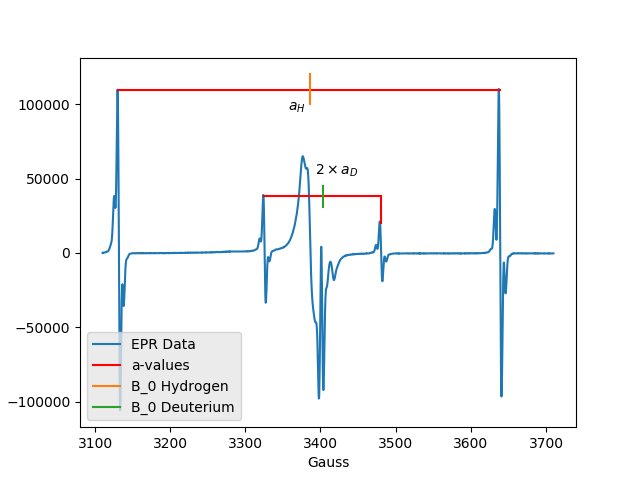
\includegraphics[scale=.8]{epr.png}
\caption{EPR spekter. De røde linjene markerer hyperfinsplittingene $a_H$ og $a_D$. Den tredje linjen til deterium ligger i midten sammen med støyen fra svovel, vi har derfor målt avstanden $a_D\times 2$ og må derfor dele denne avstanden på to for å finne $a_D$}
\end{figure}
\subsection*{5}%5
Fra målingene har vi:\\
$H_1 = 3131.8$ gauss\\
$H_2 = 3639.2$ gauss\\
$a_H = H_2 - H_1 = 507.4$ gauss = $50.74$ mT\\
$D_1 = 3325.6$ gauss\\
$D_2 = 3480.7$ gauss\\
$a_D = (D_2 - D_1)/2$ = 77.55 gauss = 7.755 mT\\
$a_H/a_D = 6.543$\\
Sammenligner vi med det teoretiske resultatet i oppgave 3.2, er dette ganske bra.

\subsection*{6}
$B_0(H) = (H_1 + H_2)/2 = 3385.5$ gauss = $338.55$ mT\\
$B_0(D) = (D_1 + D_2)/2 = 3403.15$ gauss = $340.315$ mT\\
$g_H = h\nu/\beta B_0(H) = 2.01324$\\
$g_D = h\nu/\beta B_0(D) = 2.00279$\\

Disse er ikke like på grunn av spinn-bane koblingen. Elektronets angulær moment og egenspinn vekselvirker med hverandre, noe som fører til en liten korreksjon i energinivåene.\\



\subsection*{7}
Teoretisk:\\ $|\Psi (0)|^2 = (\frac{1}{\sqrt{\pi a_0^3}}exp(0/a_0)^2 = \frac{1}{\pi a_0^3}$\\
$a_0$ er bohrradien på $0.529\times 10^{-10}$m\\
$\rightarrow |\Psi (0)|^2 = 2.15022106014e+30 m^{-3}$\\
Bare avhengig av bohrradien, og er derfor den samme for H og D\\

Eksperimentelt:\\
$|\Psi (0)|^2 = 3*a/(2\mu_0 g_N \beta)$\\
$\beta = 9.274009e-24$ J/T
$mu_0 = 1.257e-6$T*m/A
$g_N(H) = 5.585$
$g_N(D) = 0.857$
$a_H = 50.74 $mT
$a_D = 7.755$ mT

Fyller vi inn verdiene får vi \\
$|\Psi_H (0)|^2 = 1.16900334479e+27$\\
$|\Psi_D (0)|^2 = 1.16436582094e+27$\\
Aner ikke hva problemet er.
\section{Gjennomføring del b}
Vi skal ta opp EPR spektre fra tre rør med pulver av bestrålte tabletter. Disse rørene har blitt bestrålt med 68 Gy, 20 Gy og 10 Gy. Vi adderer sammen fire spektre for hver prøve. I tillegg adderer vi sammen fire spektre fra en prøve bestrålt med et ukjent mengde Gy, som skal være tilsvarende menge som ble funnet i nitroglyserin tablettene til J.L. Vi lager et kalibreringsdiagram utifra prøvene med kjente doser og benytter dette digrammet til å bestemme dosen J.L fikk under kjellerulykken.

\section{Oppgaver del b}
\subsection*{1}
\subsection*{2}
\begin{figure}[H]
\centering
\begin{tabular}{|c|c|c|}
\hline
Dose & $H_1$ & $H_2$\\
\hline
68 & $2.105\times 10^5$ & $1.078 \times 10^{5}$\\
20 & 82503 & $4.307\times 10^{4}$\\
10 & 65356 & $3.481\times 10^{4}$\\
J.L & $1.222\times 10^{5}$ & $6.575\times 10^{4}$\\
\hline
\end{tabular}
\end{figure}
\subsection*{3}
\begin{figure}[H]
\centering
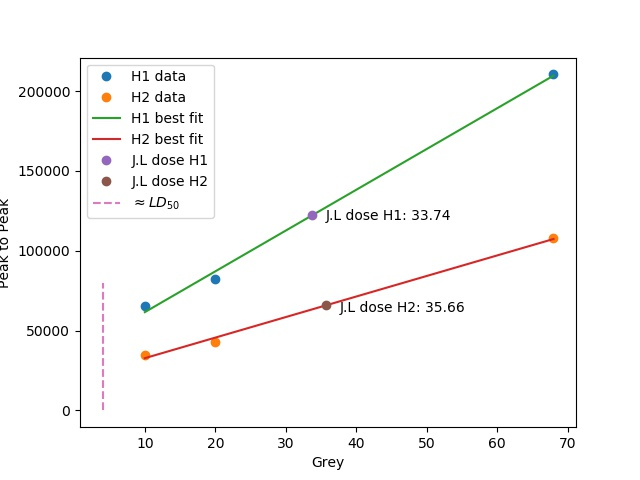
\includegraphics[scale=.6]{JL.jpg}
\end{figure}
\subsection*{4} 	
Utifra kurvene i oppgave 3 ser vi at dosen J.L fikk i seg var ca 34 Gy
\subsection*{5} 	
Siden en helkroppsdose på 10 Gy er regnet som en grense der 100 \% av befolkningen vil dø, ville det vært et medisinsk mirakel om J.L overlevde en helkroppsdose på 34 Gy

\end{document} 